\documentclass[11pt,a4paper]{article}
\usepackage[T1]{fontenc}
\usepackage[left=2cm, right=2cm, top=2cm, bottom=2cm]{geometry}
\usepackage{graphicx}
\usepackage{mathtools}
\usepackage{amssymb}
\usepackage{amsthm}
\usepackage{thmtools}
\usepackage{xcolor}
\usepackage{nameref}
\usepackage[colorlinks=true, linkcolor=blue, citecolor=cyan]{hyperref}
\usepackage{natbib} 
\usepackage{tkz-graph}
\usepackage{placeins}
\usepackage{enumerate}
\usepackage{tikz}
\usetikzlibrary{arrows}
\usepackage{tikz-cd}
\usepackage{quiver}


\newcommand{\grad}{\operatorname{grad}}
\newcommand{\curl}{\operatorname{curl}}
\renewcommand{\div}{\operatorname{div}}
\newcommand{\img}{\operatorname{img}}
\newcommand{\set}[1]{\{#1\}}
\newcommand{\R}{\mathbb{R}}

\newcommand{\Obj}{\operatorname{Obj}}
\newcommand{\Morph}{\operatorname{Morph}}


\newcommand{\boxedR}[1]{\fcolorbox{red}{white}{#1}}
\newcommand{\boxedG}[1]{\fcolorbox{green}{white}{#1}}

\newcommand{\xc}[1]{%
	\tikz[baseline=(n.base)]{
		\node[inner sep=0pt] (n) {$#1$};
		\draw[red,thick] (n.west) -- (n.east);
	}%
}



\theoremstyle{definition}
\newtheorem{definition}{Definition}
\newtheorem{prob}{Problem Statemnt}
\newtheorem{example}{Example}


\theoremstyle{remark}
\newtheorem{remark}{Remark}

\title{Hausdorff Spaces and Categorical Products}
\author{Ali Fele Paranj}



\begin{document}
	\maketitle
	
	\begin{abstract}
		Do not think too hard. This is a short note about some intuitive remarks on the Hausdorff spaces and the Categorical products, in a disjoint way!
	\end{abstract}
	
	\section{Categorical Product}
	We start with a definition.
	\begin{definition}[Categorical Product]
		Let  $ C $ be a category. ``The'' categorical product of $ X,Y \in \Obj(C) $, if it exists, is $ X\times Y \in \Obj(C) $ along with two morphisms $ \pi_1: X\times Y \to X $ and $ p_2:X\times Y \to Y $ with the following universal property: For any other $ Z\in \Obj(C) $, along with two maps $ f_1:Z\to X $ and $ f_2:Z\to Y $, there exists a unique morphism $ f: Z\to X\times Y $ such that the following diagram commutes.
		
		% https://q.uiver.app/#q=WzAsNCxbMiwxLCJYXFx0aW1lcyBZIl0sWzMsMCwiWCJdLFszLDIsIlkiXSxbMCwxLCJaIl0sWzAsMSwiXFxwaV8xIiwxXSxbMCwyLCJcXHBpXzIiLDFdLFszLDAsImYiLDEseyJzdHlsZSI6eyJib2R5Ijp7Im5hbWUiOiJkYXNoZWQifX19XSxbMywyLCJmXzIiLDEseyJjdXJ2ZSI6Mn1dLFszLDEsImZfMSIsMSx7ImN1cnZlIjotMn1dXQ==
		\[\begin{tikzcd}
			&&& X \\
			Z && {X\times Y} \\
			&&& Y
			\arrow["{f_1}"{description}, curve={height=-12pt}, from=2-1, to=1-4]
			\arrow["f"{description}, dashed, from=2-1, to=2-3]
			\arrow["{f_2}"{description}, curve={height=12pt}, from=2-1, to=3-4]
			\arrow["{\pi_1}"{description}, from=2-3, to=1-4]
			\arrow["{\pi_2}"{description}, from=2-3, to=3-4]
		\end{tikzcd} \]
		
		The categorical product of $ X $ and $ Y $ is unique up to isomorphism. In fact, more is true. They are unique up to unique isomorphism.
	\end{definition}
	
	The categorical product in the category of sets is the Cartesian product. The following is a very illustrative example of the categorical product in a very simple category.
	
	
	\begin{example}
		Let $ \mathcal{P} = (P,\leq) $ be a partially ordered set. I.e. there is a relation $ R $ on the set, dented by $ \leq $ that has the following properties:
		\begin{enumerate}[(i)]
			\item For all $ a\in P $ we have $ a\leq a $.
			\item If $ a\leq b $ and $ b\leq a $ then we should have $ a = b $. I.e. no two distinct elements precedes each other.
			\item If $ a\leq b $ and $ b\leq c $ then $ a\leq c $. 
		\end{enumerate}
		Then $ C = \mathcal{P} $ is a Category where $ \Obj(C) = P $, the underlying set, and $ \Morph(C) $ is given by
		\[ \Morph(p,q) = \set{(p,q)} \quad \text{if $ p\leq q $, otherwise $ \emptyset $}. \]
		It is easy to check that this category indeed satisfies the properties of a category. In this category, the product of two elements, is their greatest lower bound denoted by $ glb(p,q) $. To see this, it is easy to check that the following diagram commutes:
		
		% https://q.uiver.app/#q=WzAsNCxbMiwxLCJwXFx0aW1lcyBxIl0sWzMsMCwicCJdLFszLDIsInEiXSxbMCwxLCJ6Il0sWzAsMSwicFxcdGltZXMgcSBcXGxlcSBxIiwxXSxbMCwyLCJwXFx0aW1lcyBxIFxcbGVxIHEiLDFdLFszLDAsInpcXGxlcSBwXFx0aW1lcyBxIiwxLHsic3R5bGUiOnsiYm9keSI6eyJuYW1lIjoiZGFzaGVkIn19fV0sWzMsMiwielxcbGVxIHEiLDEseyJjdXJ2ZSI6Mn1dLFszLDEsInpcXGxlcSBwIiwxLHsiY3VydmUiOi0yfV1d
		\[\begin{tikzcd}
			&&& p \\
			z && {p\times q} \\
			&&& q
			\arrow["{z\leq p}"{description}, curve={height=-12pt}, from=2-1, to=1-4]
			\arrow["{z\leq p\times q}"{description}, dashed, from=2-1, to=2-3]
			\arrow["{z\leq q}"{description}, curve={height=12pt}, from=2-1, to=3-4]
			\arrow["{p\times q \leq q}"{description}, from=2-3, to=1-4]
			\arrow["{p\times q \leq q}"{description}, from=2-3, to=3-4]
		\end{tikzcd}\]
		In this context, it is customary to denote the product with $ \wedge $ symbol, i.e. write $ p\times q $ as $ p\wedge q $.
	\end{example} 
	\begin{remark}
		In the example above, if $ P $ is a family of sets, then the categorical product of $ A,B \in P $ is simply their intersection. In this context, their product is shown as $ A\cap B $.
		
		{\color{red} \noindent Important:} Notice that, in the category of sets, the categorical product is Cartesian product. However, If we consider the family of sets as a partially ordered set, then the categorical products in this category (the poset itself is a category) is the intersection.
	\end{remark}
	
	\begin{example}
		Note that the categorical product of two objects may fail to exist in genera. For example, in the category of field, for general fields, $ F_1\times F_2 $ may fail to exist.
	\end{example}
	
	Dual to the categorical product, is the idea of categorical co-product as defined below:
	
	\begin{definition}[Categorical Coproduct]
		Let $ X,Y \in \Obj(C) $ be objects in category $ C $. Their coproduct, if it exists is ``the'' object $ X\sqcup Y $ along with the morphisms $ \iota_1: X\to X\sqcup Y $ and $ \iota_2: Y\to X\sqcup Y $ (the inclusion maps), such that for any other object $ Z $ alongwith the morphisms $ f_1:X\to Z $ and $ f_2:X\to Z $, there is a unique morphism $ f:X\sqcup Y\to Z $ such that the following morphism commutes.
		
		% https://q.uiver.app/#q=WzAsNCxbMiwxLCJYIFxcc3FjdXAgWSJdLFszLDAsIlgiXSxbMywyLCJZIl0sWzAsMSwiWiJdLFsxLDAsIlxcaW90YV8xIiwxXSxbMiwwLCJcXGlvdGFfMiIsMV0sWzAsMywiZiIsMSx7InN0eWxlIjp7ImJvZHkiOnsibmFtZSI6ImRhc2hlZCJ9fX1dLFsxLDMsImZfMSIsMSx7ImN1cnZlIjozfV0sWzIsMywiZl8yIiwxLHsiY3VydmUiOi0zfV1d
		\[\begin{tikzcd}
			&&& X \\
			Z && {X \sqcup Y} \\
			&&& Y
			\arrow["{f_1}"{description}, curve={height=18pt}, from=1-4, to=2-1]
			\arrow["{\iota_1}"{description}, from=1-4, to=2-3]
			\arrow["f"{description}, dashed, from=2-3, to=2-1]
			\arrow["{f_2}"{description}, curve={height=-18pt}, from=3-4, to=2-1]
			\arrow["{\iota_2}"{description}, from=3-4, to=2-3]
		\end{tikzcd}\]
	\end{definition}
	
	In the category of sets, the coproduct of two sets is their disjoint union.
	\begin{example}
		Continuing the example above, for the partially ordered set $ \mathcal{P} $, the coproduct of $ p,q $ is their least upper bound. It is easy to check the the diagram below commutes.
		% https://q.uiver.app/#q=WzAsNCxbMiwxLCJwIFxcc3FjdXAgcSJdLFszLDAsInAiXSxbMywyLCJxIl0sWzAsMSwieiJdLFsxLDAsInBcXGxlcSBwXFxzcWN1cCBxICIsMV0sWzIsMCwicVxcbGVxIHBcXHNxY3VwIHEiLDFdLFswLDMsInBcXHNxY3VwIHEgXFxsZXEgeiIsMSx7InN0eWxlIjp7ImJvZHkiOnsibmFtZSI6ImRhc2hlZCJ9fX1dLFsxLDMsInBcXGxlcSB6IiwxLHsiY3VydmUiOjN9XSxbMiwzLCJxXFxsZXEgeiIsMSx7ImN1cnZlIjotM31dXQ==
		\[\begin{tikzcd}
			&&& p \\
			z && {p \sqcup q} \\
			&&& q
			\arrow["{p\leq z}"{description}, curve={height=18pt}, from=1-4, to=2-1]
			\arrow["{p\leq p\sqcup q }"{description}, from=1-4, to=2-3]
			\arrow["{p\sqcup q \leq z}"{description}, dashed, from=2-3, to=2-1]
			\arrow["{q\leq z}"{description}, curve={height=-18pt}, from=3-4, to=2-1]
			\arrow["{q\leq p\sqcup q}"{description}, from=3-4, to=2-3]
		\end{tikzcd}\]
	\end{example}
	
	
	\begin{remark}
		It is not uncommon, when one reads the notion of disjoint union of sets for the first time, they notice some sort of similarity between that construct and the direct sum of vector spaces. The whole idea of category theory is to ``build'' appropriate consistent stories that reflects the felt similarities between the objects, so that people can communicate about these kind of feelings without ambiguity.
	\end{remark}
	
	
	
	\begin{remark}[My Confusion]
		It is fairly clear that the co-product in the case of vector spaces is the direct sum $ V_1\oplus V_2 $, and their product $ \sqcap_{i=1}^2 V_i $ is isomorphic to their direct sum. However, in the case of infinitely many vector spaces, their direct product is not isomorphic to their direct sum. Why?
	\end{remark}
	
	
	\section{Hausdorff Spaces}
	In this section, I will give some intuitions about the Hausdorff spaces. A Topological space is Hausdorff if for any two points there disjoint open sets that separates them. It is very easy to see not unique limit implies not Hausdorff (the two limiting points can not be seperated by open sets). The line with two origins is a very useful way to think about this. As depicted below, a line with two origins can be constructed by the quotient structure $ A\cup B / \sim $ where $ \sim $ is a relation on $ A\cup B $ where $ (x_A,1) \sim (x_B,-1) $ if $ x_A=x_b \neq 0 $. The open sets in this quotient space are the images of the open sets in $ A\cup B $ (note that $ A\cup B \subset \R^2 $ inherits the subspace topology of $ \R^2 $, where $ \R^2 $ itself inherits the product topology of $ \R $). So all open sets in $ X $ will contain both versions of $ 0 $, thus there is no open sets that can distinguish $ 0^+ $ and $ 0^- $. This also can be seen by considering the sequence $ (1/n)_n $. This sequence converges to both $ 0^+ $ and $ 0^- $. So the space is not Hausdorff.
	
	\begin{figure}[h!]
	\centering
	
	
	
	\tikzset{every picture/.style={line width=0.75pt}} %set default line width to 0.75pt        
	
	\begin{tikzpicture}[x=0.75pt,y=0.75pt,yscale=-1,xscale=1]
		%uncomment if require: \path (0,300); %set diagram left start at 0, and has height of 300
		
		%Straight Lines [id:da969765889597233] 
		\draw    (70,130) -- (288,130) ;
		\draw [shift={(290,130)}, rotate = 180] [color={rgb, 255:red, 0; green, 0; blue, 0 }  ][line width=0.75]    (10.93,-3.29) .. controls (6.95,-1.4) and (3.31,-0.3) .. (0,0) .. controls (3.31,0.3) and (6.95,1.4) .. (10.93,3.29)   ;
		%Straight Lines [id:da664250379178352] 
		\draw    (170,200) -- (170,52) ;
		\draw [shift={(170,50)}, rotate = 90] [color={rgb, 255:red, 0; green, 0; blue, 0 }  ][line width=0.75]    (10.93,-3.29) .. controls (6.95,-1.4) and (3.31,-0.3) .. (0,0) .. controls (3.31,0.3) and (6.95,1.4) .. (10.93,3.29)   ;
		%Straight Lines [id:da05235119937722865] 
		\draw [color={rgb, 255:red, 74; green, 144; blue, 226 }  ,draw opacity=1 ]   (80,100) -- (270,100) ;
		%Straight Lines [id:da04194615510817612] 
		\draw [color={rgb, 255:red, 74; green, 144; blue, 226 }  ,draw opacity=1 ]   (80,160) -- (270,160) ;
		%Straight Lines [id:da6559753598643184] 
		\draw [color={rgb, 255:red, 74; green, 144; blue, 226 }  ,draw opacity=1 ][line width=2.25]    (380,130) -- (570,130) ;
		%Shape: Circle [id:dp06752199537396808] 
		\draw  [color={rgb, 255:red, 74; green, 144; blue, 226 }  ,draw opacity=1 ][line width=2.25]  (471.75,126.75) .. controls (471.75,124.96) and (473.21,123.5) .. (475,123.5) .. controls (476.79,123.5) and (478.25,124.96) .. (478.25,126.75) .. controls (478.25,128.54) and (476.79,130) .. (475,130) .. controls (473.21,130) and (471.75,128.54) .. (471.75,126.75) -- cycle ;
		%Shape: Circle [id:dp0037727303722537853] 
		\draw  [color={rgb, 255:red, 74; green, 144; blue, 226 }  ,draw opacity=1 ][line width=2.25]  (471.75,132.75) .. controls (471.75,130.96) and (473.21,129.5) .. (475,129.5) .. controls (476.79,129.5) and (478.25,130.96) .. (478.25,132.75) .. controls (478.25,134.54) and (476.79,136) .. (475,136) .. controls (473.21,136) and (471.75,134.54) .. (471.75,132.75) -- cycle ;
		
		% Text Node
		\draw (45,72.4) node [anchor=north west][inner sep=0.75pt]    {$A\ =\mathbb{R} \times \{1\}$};
		% Text Node
		\draw (41,162.4) node [anchor=north west][inner sep=0.75pt]    {$B\ =\mathbb{R} \times \{-1\}$};
		% Text Node
		\draw (541,102.4) node [anchor=north west][inner sep=0.75pt]    {$A\cup B/\sim $};
		
		
	\end{tikzpicture}
\end{figure}
	\FloatBarrier
	
	Another characterization of a Hausdorff space is having closed diagonal $ \Delta = \set{(x,x)\in X\times X} $. It is straight forward to show that having a closed diagonal is equivalent to being Hausdorff. For the line with two origins example above the diagonal will be
	\begin{figure}[h!]
	\centering
	
	
	
	\tikzset{every picture/.style={line width=0.75pt}} %set default line width to 0.75pt        
	
	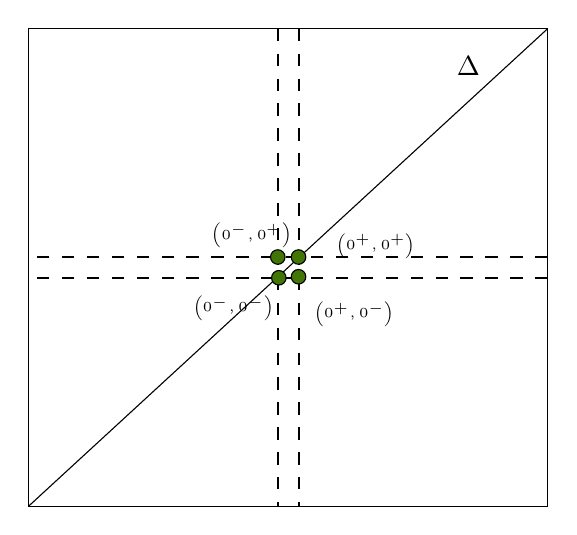
\begin{tikzpicture}[x=0.75pt,y=0.75pt,yscale=-1,xscale=1]
		%uncomment if require: \path (0,300); %set diagram left start at 0, and has height of 300
		
		%Shape: Rectangle [id:dp5193643571266664] 
		\draw   (150,20) -- (400,20) -- (400,250) -- (150,250) -- cycle ;
		%Straight Lines [id:da2432122097230004] 
		\draw [color={rgb, 255:red, 0; green, 0; blue, 0 }  ,draw opacity=1 ][line width=0.75]  [dash pattern={on 4.5pt off 4.5pt}]  (270,20) -- (270,250) ;
		%Straight Lines [id:da8789847469102436] 
		\draw [color={rgb, 255:red, 0; green, 0; blue, 0 }  ,draw opacity=1 ][line width=0.75]  [dash pattern={on 4.5pt off 4.5pt}]  (280,20) -- (280,250) ;
		%Straight Lines [id:da6533899359137522] 
		\draw [color={rgb, 255:red, 0; green, 0; blue, 0 }  ,draw opacity=1 ][line width=0.75]  [dash pattern={on 4.5pt off 4.5pt}]  (400,130) -- (150,130) ;
		%Straight Lines [id:da535776408423082] 
		\draw [color={rgb, 255:red, 0; green, 0; blue, 0 }  ,draw opacity=1 ][line width=0.75]  [dash pattern={on 4.5pt off 4.5pt}]  (400,140) -- (150,140) ;
		%Straight Lines [id:da5554446790214769] 
		\draw    (400,20) -- (150,250) ;
		%Shape: Circle [id:dp32546629561587426] 
		\draw  [fill={rgb, 255:red, 65; green, 117; blue, 5 }  ,fill opacity=1 ] (276.5,130) .. controls (276.5,128.07) and (278.07,126.5) .. (280,126.5) .. controls (281.93,126.5) and (283.5,128.07) .. (283.5,130) .. controls (283.5,131.93) and (281.93,133.5) .. (280,133.5) .. controls (278.07,133.5) and (276.5,131.93) .. (276.5,130) -- cycle ;
		%Shape: Circle [id:dp8202919592455564] 
		\draw  [fill={rgb, 255:red, 65; green, 117; blue, 5 }  ,fill opacity=1 ] (266.5,130) .. controls (266.5,128.07) and (268.07,126.5) .. (270,126.5) .. controls (271.93,126.5) and (273.5,128.07) .. (273.5,130) .. controls (273.5,131.93) and (271.93,133.5) .. (270,133.5) .. controls (268.07,133.5) and (266.5,131.93) .. (266.5,130) -- cycle ;
		%Shape: Circle [id:dp7704702433707692] 
		\draw  [fill={rgb, 255:red, 65; green, 117; blue, 5 }  ,fill opacity=1 ] (276.5,139.5) .. controls (276.5,137.57) and (278.07,136) .. (280,136) .. controls (281.93,136) and (283.5,137.57) .. (283.5,139.5) .. controls (283.5,141.43) and (281.93,143) .. (280,143) .. controls (278.07,143) and (276.5,141.43) .. (276.5,139.5) -- cycle ;
		%Shape: Circle [id:dp40492667019933914] 
		\draw  [fill={rgb, 255:red, 65; green, 117; blue, 5 }  ,fill opacity=1 ] (267,140) .. controls (267,138.07) and (268.57,136.5) .. (270.5,136.5) .. controls (272.43,136.5) and (274,138.07) .. (274,140) .. controls (274,141.93) and (272.43,143.5) .. (270.5,143.5) .. controls (268.57,143.5) and (267,141.93) .. (267,140) -- cycle ;
		
		% Text Node
		\draw (297,117.4) node [anchor=north west][inner sep=0.75pt]  [font=\tiny,color={rgb, 255:red, 0; green, 0; blue, 0 }  ,opacity=1 ]  {$\left( 0^{+} ,0^{+}\right)$};
		% Text Node
		\draw (286.5,150.4) node [anchor=north west][inner sep=0.75pt]  [font=\tiny,color={rgb, 255:red, 0; green, 0; blue, 0 }  ,opacity=1 ]  {$\left( 0^{+} ,0^{-}\right)$};
		% Text Node
		\draw (228,147.4) node [anchor=north west][inner sep=0.75pt]  [font=\tiny,color={rgb, 255:red, 0; green, 0; blue, 0 }  ,opacity=1 ]  {$\left( 0^{-} ,0^{-}\right)$};
		% Text Node
		\draw (237,112.4) node [anchor=north west][inner sep=0.75pt]  [font=\tiny,color={rgb, 255:red, 0; green, 0; blue, 0 }  ,opacity=1 ]  {$\left( 0^{-} ,0^{+}\right)$};
		% Text Node
		\draw (355,32.4) node [anchor=north west][inner sep=0.75pt]    {$\Delta $};
		
		
	\end{tikzpicture}
\end{figure}
	\FloatBarrier
	It is easy to see that $ \Delta $ is not closed in the product topology. That is because it does not contain all of its limit points, namely, it does not contain $ (0^+,0^-) $ and $ (0^-,0^+) $.
	
	
	
	
\end{document}